\chapter{Survey Text and Post-Processing}
\label{surveyappendix}

\section{Question Coding and Post-Processing}

This section presents the coding rules and rationale for survey post-processing.

\subsection{Mission Area}

In order to characterize survey respondents according to comparable mission areas, I clustered responses to the open-ended demographic question \say{On what mission does your organization spend the most time and money?}  Respondents provided 300 unique answers, and so I clustered the responses into comparable general and specific mission areas.

When clustering the responses, I divided up the answers into two categories: those who answered with an operational summary of the management tasks that they face and those who responded with the organization's activities.  For those that responded substantively about the mission, I clustered the responses into nine general categories: Animal Welfare, Arts and Culture, Environment, International, Domestic Social, Religious, Health, Education, Religious, and Other.  The distribution of mission types can be seen in Table~\ref{tab:clusterprops}. 
 \begin{table}[ht]
 \centering
 \begin{tabular}{rlrr}
   \hline
  & Cluster Theme & Number & Response Percentages \\
   \hline
 1 & Animal Welfare &   3 & 0.90\% \\
   2 & Arts and Culture &  12 & 3.80\% \\
   3 & Education &  18 & 5.60\%\\
   4 & Environmental &   6 & 1.90\% \\
   5 & Health &  22 & 6.90\% \\
   6 & International &   9 & 2.80\% \\
   7 & Operational & 137 & 42.90\% \\
   8 & Other &   3 & 0.90\% \\
   9 & Religious &  17 & 5.30\% \\
   10 & Social &  92 & 28.80\% \\
    \hline
 \end{tabular}
\caption{Distribution of General Mission Themes}
\label{tab:clusterprops}
 \end{table}
 
After classifying the reported mission areas, the \say{Domestic Social} and \say{Health} categories were populous enough to warrant additional subcategories. These subcategories are given in Table~\ref{tab:socmissions} and Table~\ref{tab:healthareas}

\begin{table}[ht]
\centering
 \begin{tabular}{lrr}
   \hline
  Cluster & Frequency & Percentage \\
   \hline
 Elderly and disabilities &  10 & 11.20\% \\
   Housing &  14 & 15.70\% \\
   Hunger &   5 & 5.60\% \\
   Other &  31 & 34.80\% \\
  Recreation &   3 & 3.40\% \\
    Violence\/crime &   2 & 2.20\% \\
 Vocational &   3 & 3.40\% \\
   Youth &  21 & 23.60\% \\
    \hline
 \end{tabular}
 \caption{Mission subcategories in Social Services Organizations}
 \label{tab:socmissions}
 \end{table}
 
  \begin{table}[ht]
 \centering
 \begin{tabular}{lrr}
   \hline
  Cluster & Number & Percent of Responses \\
   \hline
 Addictions &   1 & 4.50 \\
 Mental health &   4 & 18.20 \\
 Physical health &   9 & 40.90 \\
  Other &   8 & 36.40 \\
    \hline
 \end{tabular}
 \caption{Subcategories in Health Organizations}
 \label{tab:healthareas}
 \end{table}
 
In addition to substantive mission areas, approximately 40\% of the respondents listed teh  which I named broadly as \say{Operational}, staffing, finances, and outreach or expansion were common responses. After evaluating the responses, I clustered specific answers into common categories of answers in the responses. These are presented in Table~\ref{tab:activityareas}.

 \begin{table}[ht]
 \centering
 \begin{tabular}{lrr}
   \hline
 Activities & Number & Response Percentages \\
   \hline
  Administration &   2 & 1.50\% \\
    Don’t know &   8 & 5.80\% \\
   Finances &  14 & 10.20\% \\
   Growth &   9 & 6.60\% \\
  Infrastructure &   2 & 1.50\% \\
  Membership &   2 & 1.50\% \\
   Operations &  65 & 47.40\% \\
   Other &   4 & 2.90\% \\
   Outreach &  17 & 12.40\% \\
    Staffing &  14 & 10.20\% \\
    \hline
 \end{tabular}
 \caption{Clustering of Activities Described in Operational Responses}
 \label{tab:activityareas}
 \end{table}

\subsection{Question: Organization Size}

In order to identify the size of the organization that the respondents worked within, the survey asked respondents \say{What is the approximate number of people in your organization?}. After converting the free-text answer into an integer, I clustered the answers into seven bins ranging, from 0-2 to over 100 people. The bin sizes increase as the number of reported personnel increases, with three bins for a size of less than 10, and then one for 11-20, one for 21-50, one for 51-100, and one for any reporting over 100. The rationale for this categorization is twofold: the reported sizes exhibits a long tail, with over 200 of the 298 responses reporting a size of less than 10 people. The distribution of reported personnel sizes for those organizations reporting 100 or fewer people in the organization is displayed in Figure~\ref{fig:censoredsizes}.

%% Here put the box plot of size (and then one zoomed in)

\begin{table}
\centering
\begin{tabular}{cc}
    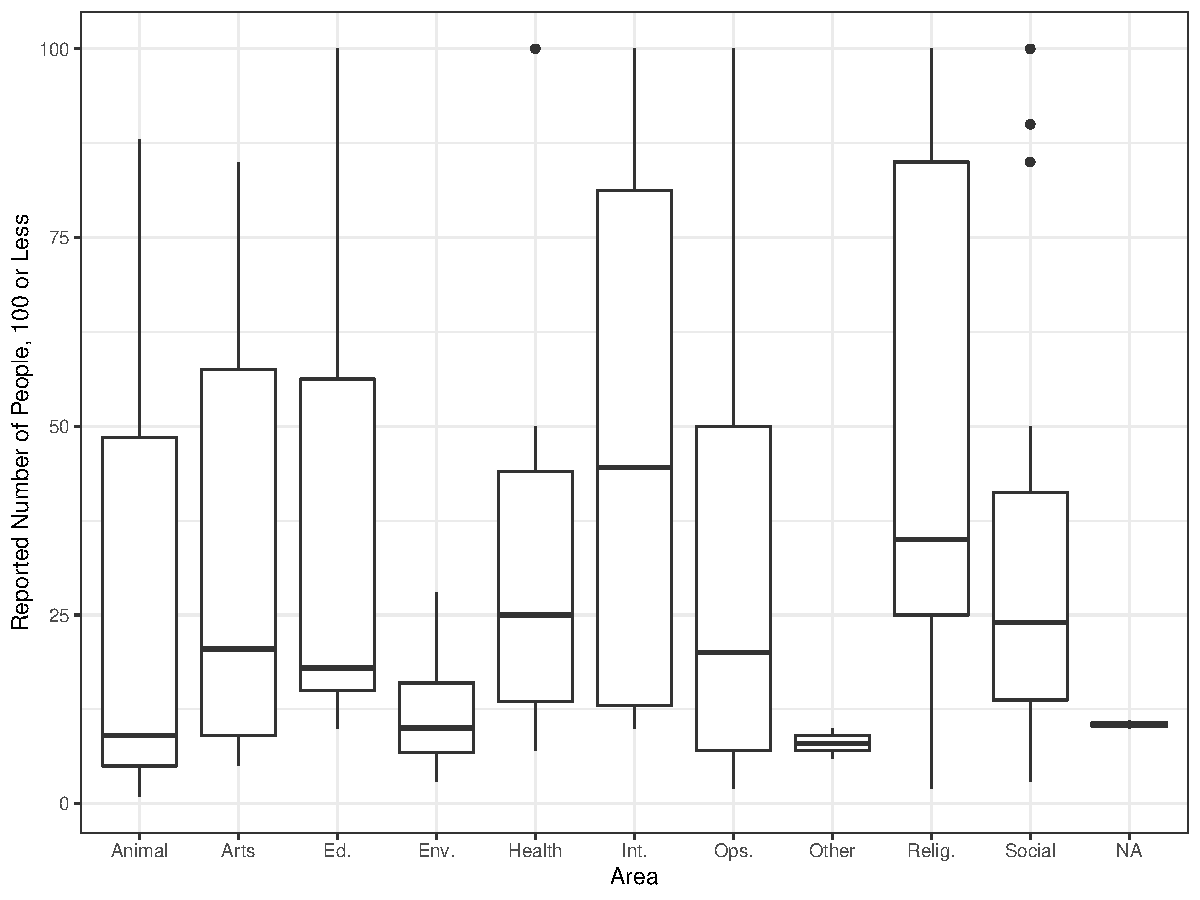
\includegraphics[width=.45\columnwidth]{./Pictures/censoredsizebysector.pdf}
&
    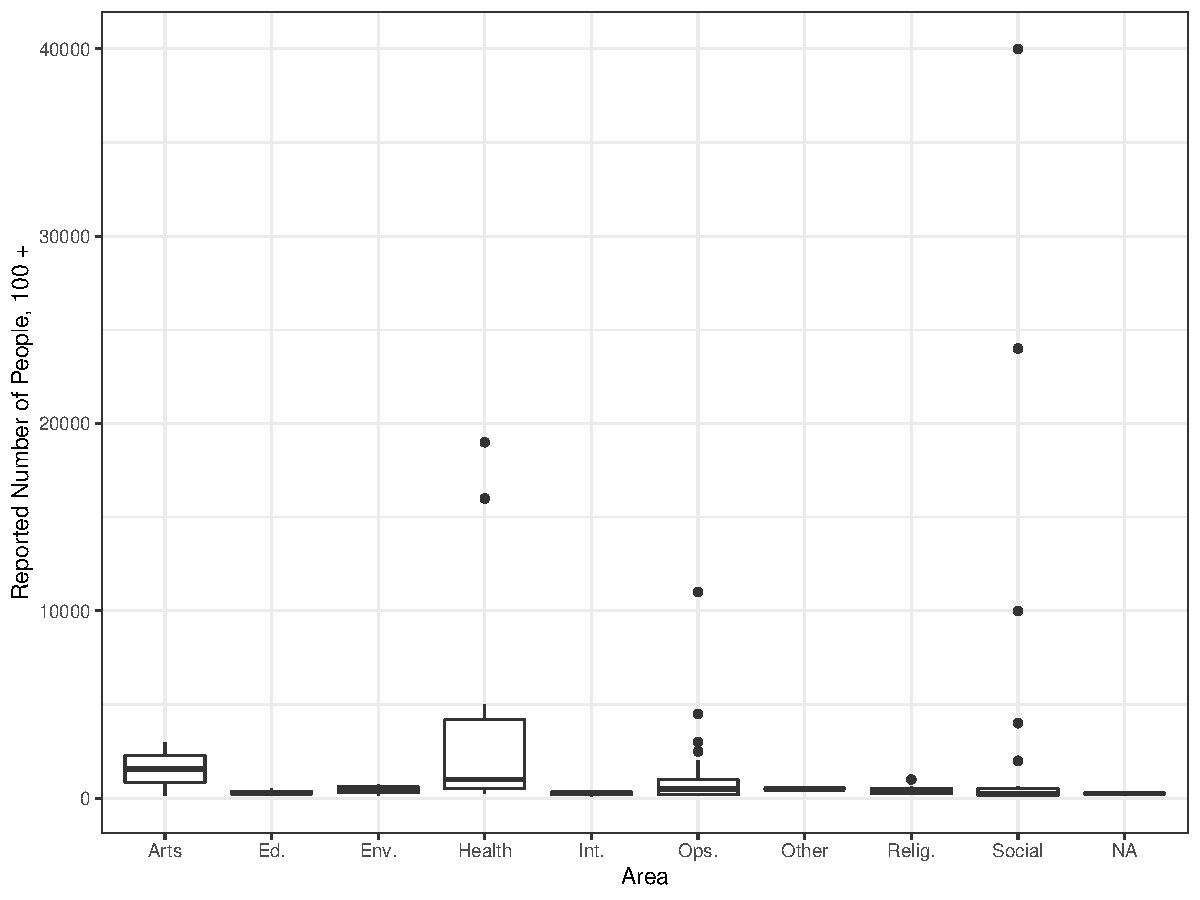
\includegraphics[width=.45\columnwidth]{./Pictures/censoredsizebysectorbig.pdf}
\\
Size $\leq$ 100 &  Size $> 100 $ \\
\end{tabular}
    \caption{Distribution of Reported Personnel Sizes}
    \label{fig:censoredsizes}
\end{table}



The expectation that smaller organizations would have less bandwidth to absorb a large influx of new staff also informed the decision to summarize the results with a more precise focus on smaller organizations.

It is more common for surveys of non-profits to classify size of the non-profit according to the size of the operating budget. Instead of following this format, the survey asked for personnel size because the project is interested in rapid staff expansions. Despite the difference in substantive focus, budget and the number of full-time employees are strongly correlated~\autocite{carman2009nonprofits}.  

\subsection{Descriptions of Origin of Post-Expansion Mission Drift}

In order to estimate the overall frequency of expansion-driven change among the non-profit respondents, the survey posed a three part question. The sequence began with the question: \say{Have you have ever been part of an organization experiencing a period of rapid growth or personnel change among the staff or the board of directors?}. The distribution of responses reporting a rapid staff growth are displayed in Figure~\ref{fig:q13staffsummary} For those who responded in the affirmative, the survey asked the follow-up question: \say{Did you feel that the personnel changes contributed to mission drift or other strategic changes?}. The result of the question, disaggregated by reported size and clustered mission area are shown in Figure~\ref{fig:q14summary}. Finally, the survey asked for open-ended reflection on where the respondent believed that the changes originated. The question asked: \say{In a sentence or two, can you describe where the changes originated?} 

\begin{figure}
\centering
    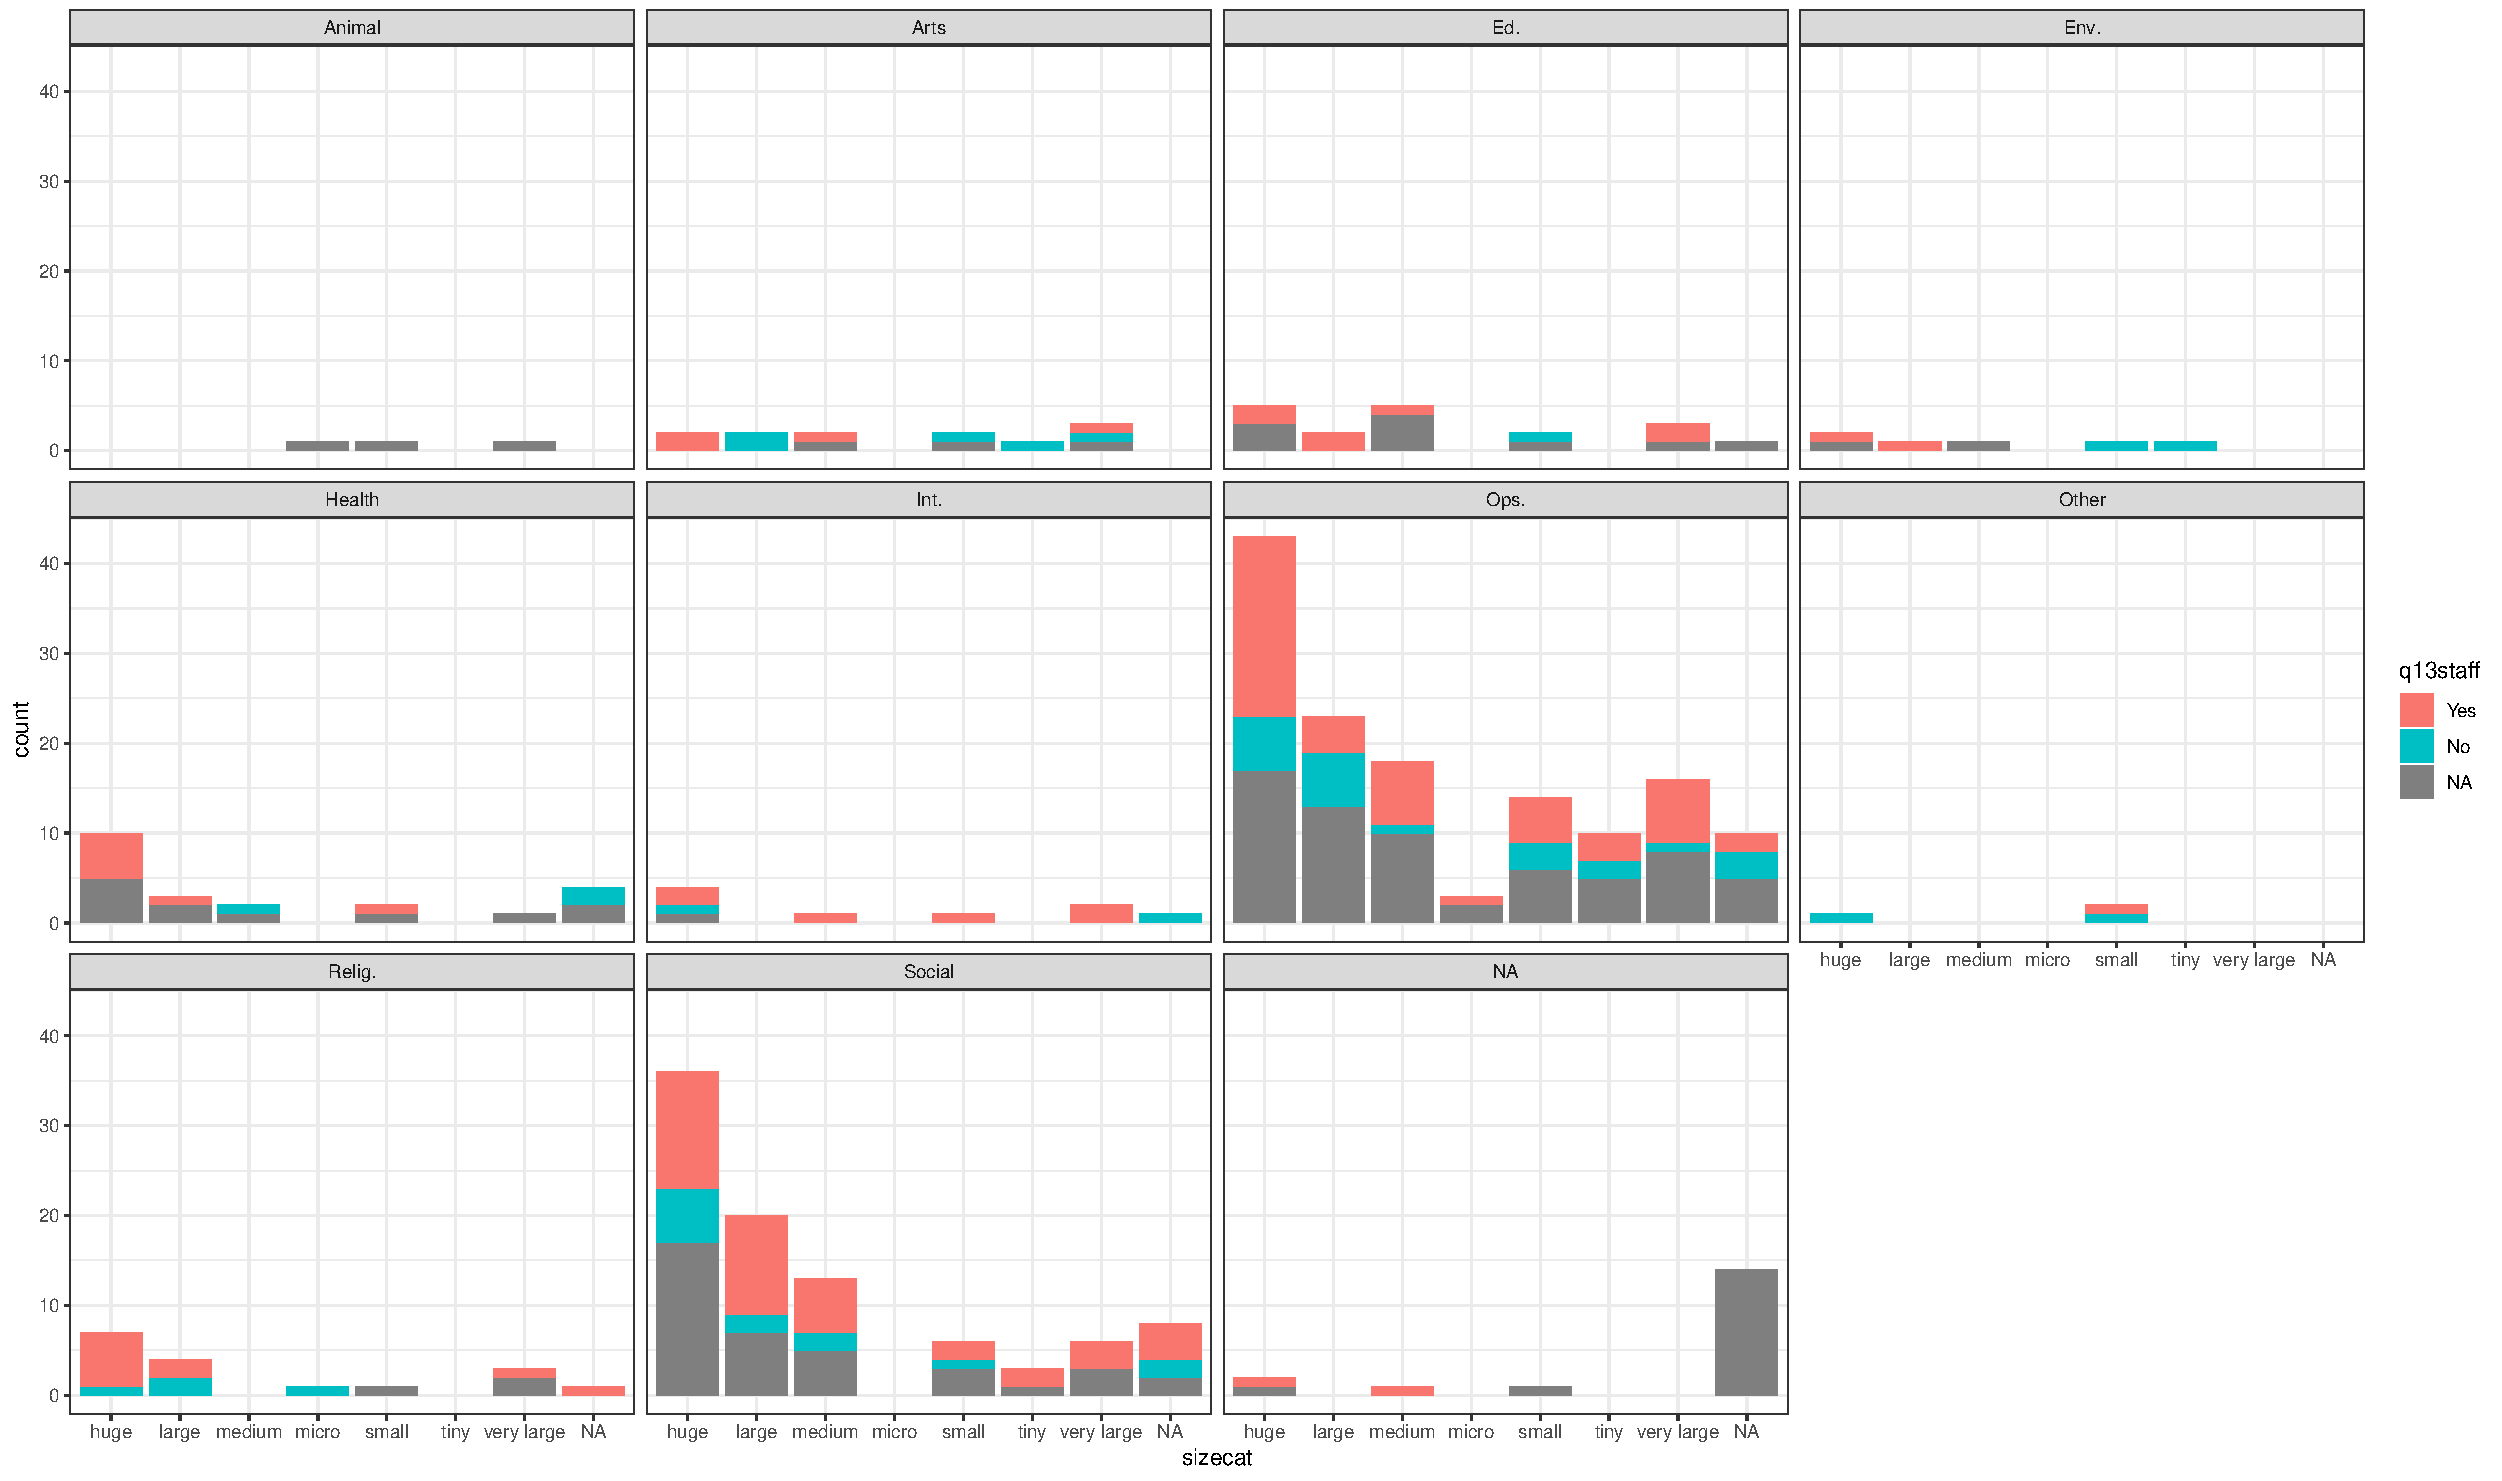
\includegraphics[width=.85\columnwidth]{./Pictures/rapidstaffgrowthbysizeandsector.pdf}
    \caption{Reports of Rapid Staff Expansion, By Size Category and Mission Cluster}
    \label{fig:q13staffsummary}
\end{figure}


\begin{figure}
\centering
    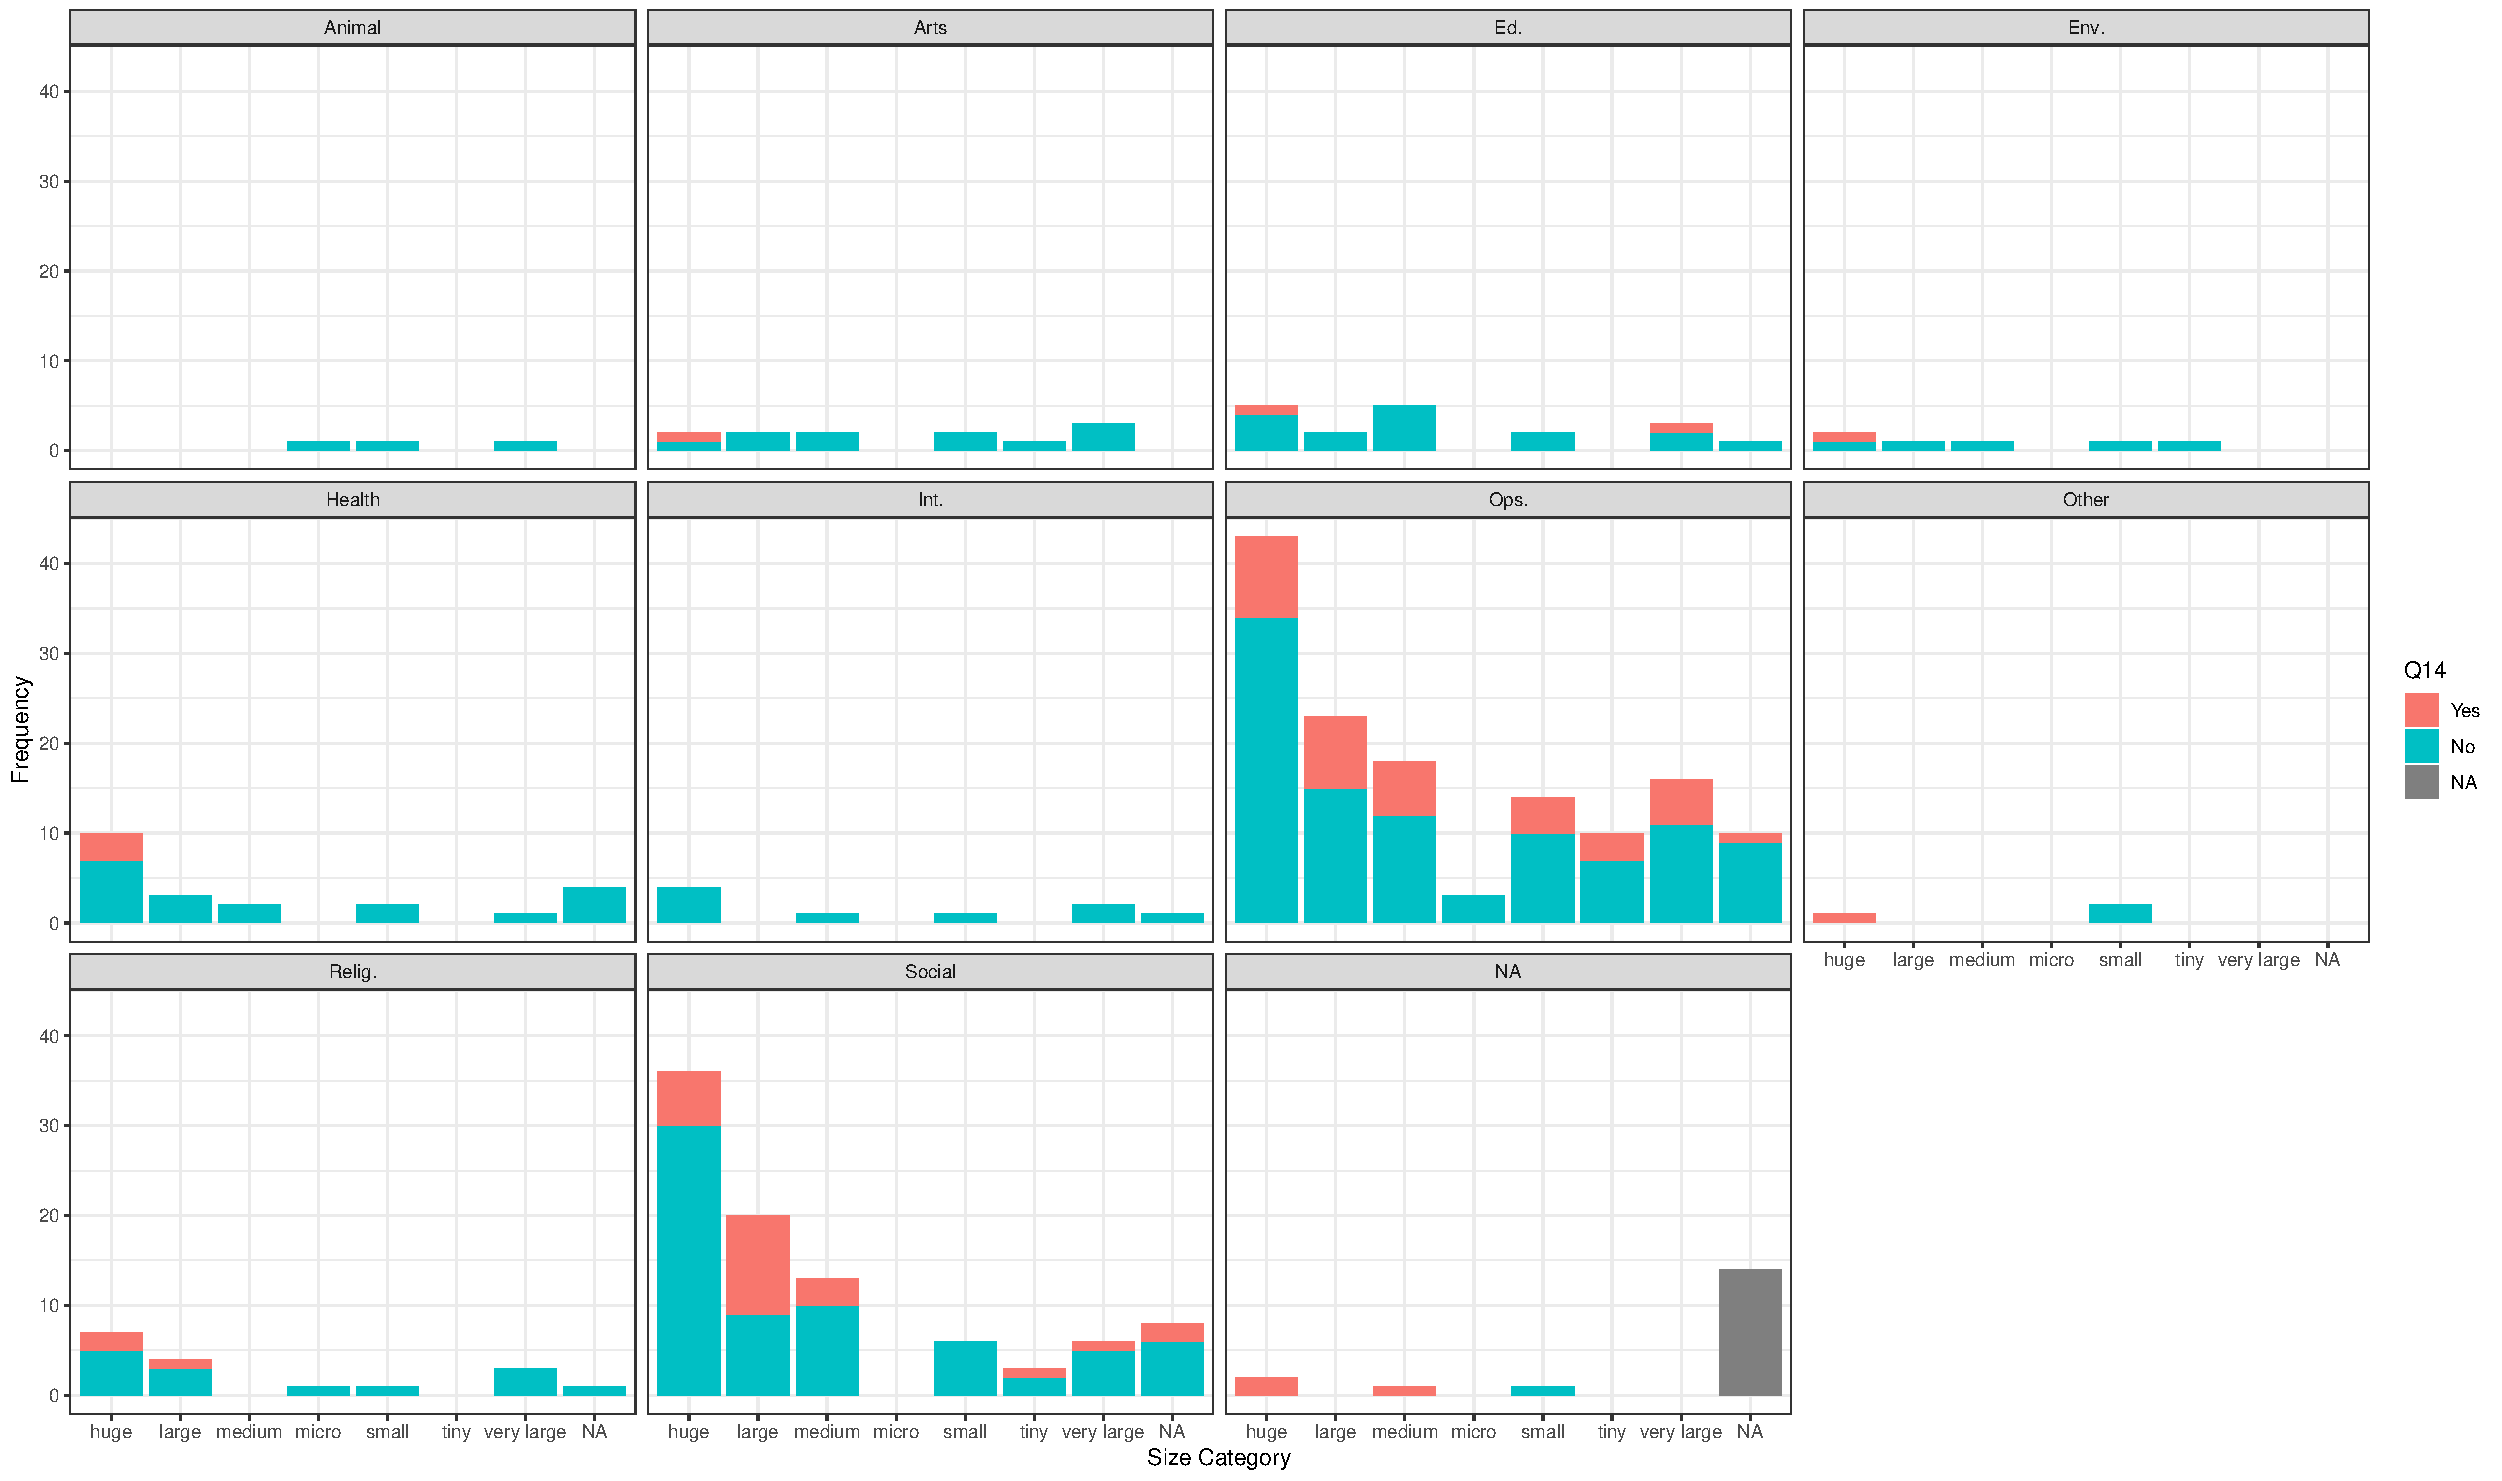
\includegraphics[width=.85\columnwidth]{./Pictures/missiondriftaftergrowth.pdf}
    \caption{Reports of Mission Drift After Rapid Growth, By Size Category and Mission Cluster}
    \label{fig:q14summary}
\end{figure}
% summary of yeses by mission category for question 13; 14; 

For the analysis, I standardized the responses, clustering them into seven general categories: no change reported; change originating from the top-down with the Board of Directors, executive officers, or general leaders;  change originating from the bottom-up and instigated by staff; change motivated by shifting demographics of the membership base or in the services provided; change originating from financial necessity; and a general category for an origin of change that did not fall into the existing categories. Finally, two residual categories noted, respectively, a cluster of answers that described a tactical motivator for change, and another in which respondents reported a technical glitch in the survey flow.\footnote{These responses were removed from the series of questions about expansion and subsequent change, so that the platform problem did not influence overall results.}

%% summary of some of the free text answers in question 16

\subsection{Descriptions of Result of Short-Term Changes}  

The bottom-up transformation theory rests on a claim that even strategic leaders can be induced to downplay long-term best practices in favor of a short-term gain or advantage. To provide an empirical basis for this assertion, the survey asked respondents \say{Have the leaders of your organization ever decided to strengthen the morale and cohesion of your organization in the short-term, even if the decision might influence the long-term strategy?} For those who answered in the affirmative, the survey provided an open-ended followup question: \say{In a sentence or two, can you describe the result of this decision?}

To standardize the responses for analysis, I clustered the free-responses into five general outcomes. The substantive clusters classified responses into whether they reported a positive or negative outcome. Reported positive outcomes frequently described reinvigorated staff, better recruiting, and a recommitment to the original mission. Conversely, the negative responses gathered responses that reported leaders pushed out or resigning, mission drift, disconnects between leaders and the base, and an overall reduction in quality of staff or services.  A  third cluster of responses indicated that they were still experiencing the fallout of the short-term changes, and so were unable to report yet. Finally, the three residual categories collected responses that indicated that the respondent had not experienced that type of outcome; did not know the results or understand the question; or that they shared advice for managing morale or retrenching against mission drift.

\section{Additional Graphs from Conjoint Experiment}

The conjoint experiment posed two hypothetical hiring scenarios to survey respondents, asking them to compare which of two candidates for a staff and a Board of Directors position they would prefer to hire. For both vignettes, the candidates were named \say{Candidate A} and \say{Candidate B,} with \say{Candidate A} being the option with varying traits.

The staff recruitment vignette presented respondents with the prompt:

\begin{quote}
Imagine you are recruiting new staff for a hypothetical organization similar to your own. The organization's funding is: \textit{{[Resource Condition]}}
There are two groups of equally well-qualified candidates:\\
Candidates in \textbf{Group A} have a mission that is \textit{{[Agreement Condition]}} the organization's mission. You expect that if they join, they will try to steer the organization's mission to align with their goals. However, there is a large foundation running a fellowship program that will subsidize their salary and benefits at \textit{{[Subsidy Condition]}}\\
Candidates in \textbf{Group B} share a mission with the organization. They are not eligible for the subsidy, and so their salary and benefits will be borne solely by the organization.\\
The candidate profiles are summarized below.\\
Drawing from your professional experience, from which group of candidates would you prefer to recruit staff?
\end{quote}

Respondents were then presented with a Board member recruitment vignette, which asked them to engage with the following scenario:

\begin{quote}
Now imagine you are recruiting a new board member for an organization similar to your own. The organization's funding is: \textit{{[Resource Condition]}}
There are two equally well-qualified candidates for the board:\\

\textbf{Candidate 1}: prefers a mission that is \textit{{[Agreement Condition]}} the organization that is seeking a board member.  The candidate \textit{{[Skills Condition]}} bring new professional skills that the board needs. You expect that if they join the board, they will try to steer the organization towards their mission.

\textbf{Candidate 2}: shares the same mission as the organization and so you do not expect them to try to change the organization's mission. They will not bring new professional skills to the board.\\
Which of the two candidates would you prefer to have on the board of directors?
\end{quote}

As Figure~\ref{fig:traitssector} indicates, the respondents largely responded similarly regardless of the sector or type of mission that they reported engaging in. Those respondents reporting activity in the \say{social} sector were the most averse to candidates with divergent preferences. But, otherwise, the response patterns are broadly similar, and therefore the responses were analyzed without differentiating the reported mission.

\begin{figure}
\centering
    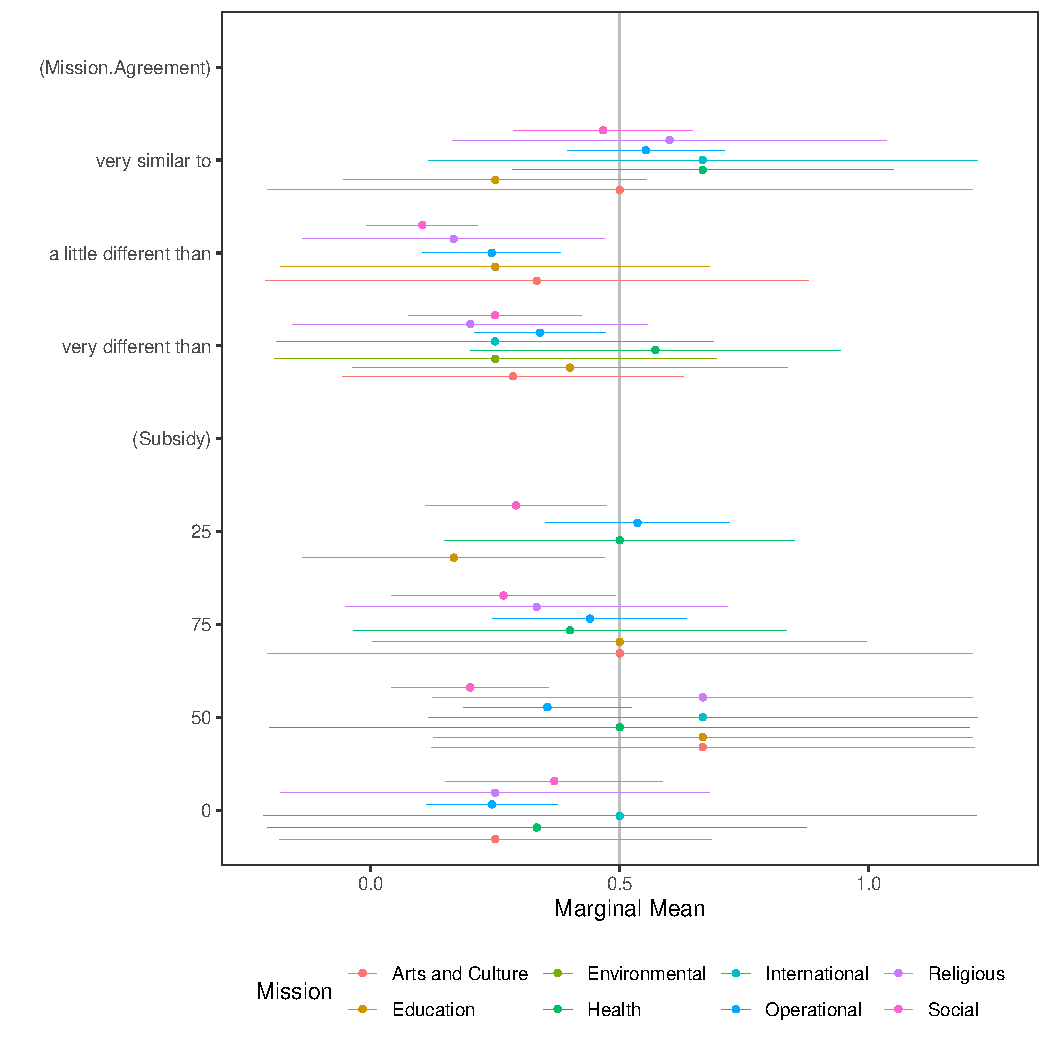
\includegraphics[width=.95\columnwidth]{./Pictures/traitsBySector.pdf}
    \caption{Trait Attractiveness By Respondent Sector}
    \label{fig:traitssector}
\end{figure}

Estimating the Average Marginal Effects by looping over the feature levels for each possible reference category for the candidate traits indicates that the estimated outcome is not sensitive to the choice of reference category. Indeed, the results of the sensitivity analysis, shown in Figure~\ref{fig:acmesens} are consistent with the overall takeaway that conjoint survey participants paid most attention to mission alignment.


\begin{figure}
\centering
    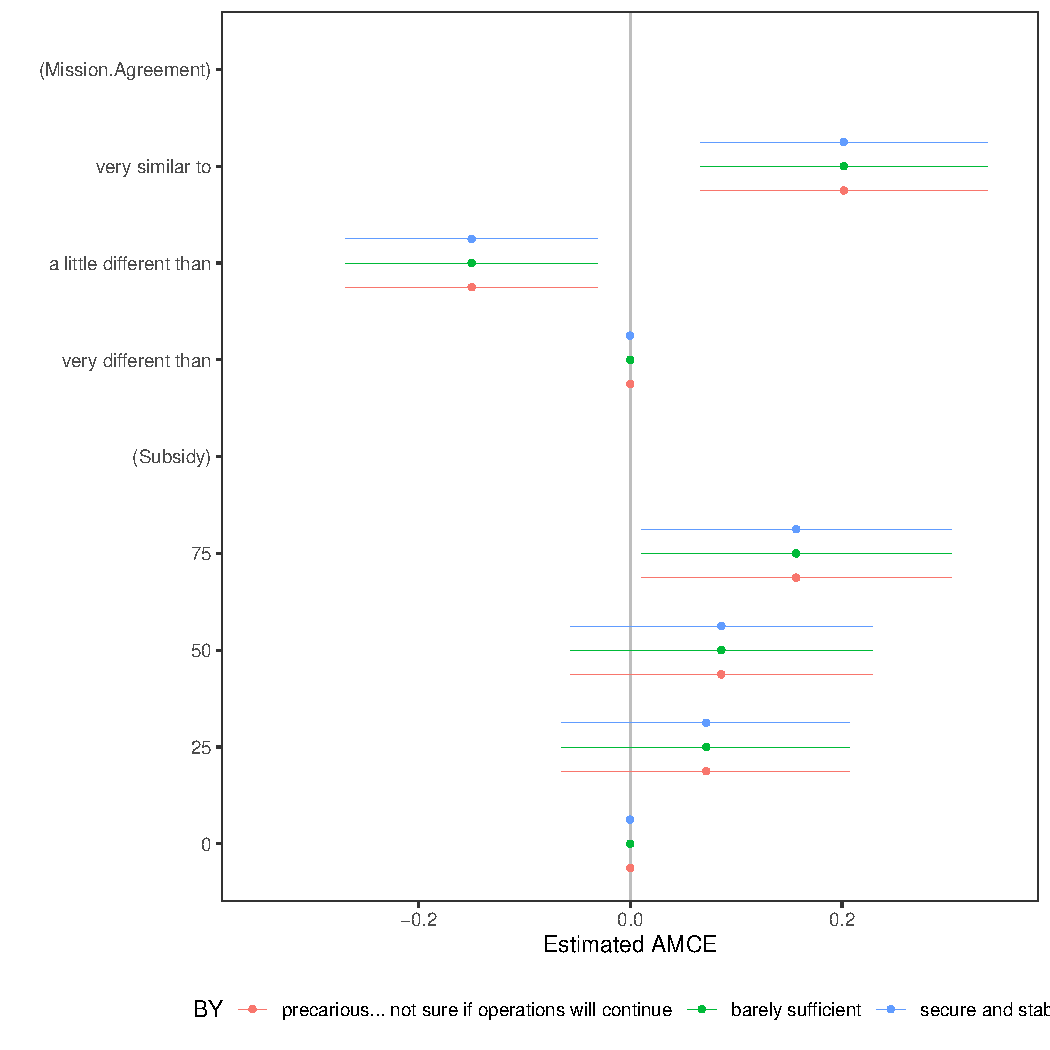
\includegraphics[width=.95\columnwidth]{./Pictures/acmeSensitivity.pdf}
    \caption{ACME Sensitivity Plot}
    \label{fig:acmesens}
\end{figure}


%% summaries of the classification for Q21.

